\documentclass[a4paper,14pt,titlepage]{article}

\usepackage[utf8]{inputenc}
\usepackage[pdftex]{graphicx}
\usepackage{polski}
\usepackage{amsfonts}
\usepackage{verbatim}
\usepackage{indentfirst}
\usepackage{listings}
\usepackage{color}

\newcommand{\TODO}{\textbf{TODO}}

% wyroznienie slow kluczowych
\newcommand{\tech}{\texttt}
%nazwy programow w tekscie -zuz
\newcommand{\prog}{\texttt}
%nazwy miar-jakosci -zuz
\newcommand{\qm}{\textit}
%wielowyrazowe nazwy ktore trzeba wyroznic
\newcommand{\name}{\textsl}

\def\notka#1{\marginpar{\tiny\bf (#1)}}

\lstset{
language=Java,
numbers=left,
frame = single,
breaklines=true,
literate={:=}{{$\gets$}}1 {<=}{{$\leq$}}1 {>=}{{$\geq$}}1 {<>}{{$\neq$}}1,
emph={[1]foreach, end, procedure, is, in},emphstyle={[1]\textbf},
emph={[2]markSubdNodes, renumberNodes, createNewMesh, joinResultNodes, joinResultElements, getBoundaryNodes, createListOfFaces, sortNodesInFaces, sortFaces}, emphstyle={[2]\textsl}
}
\definecolor{light-gray}{gray}{0.985}
\definecolor{dark-gray}{gray}{0.10}
\lstnewenvironment{code}{\lstset{language=c++,basicstyle=\ttfamily\scriptsize,numbers=right, numbersep=-20pt, xleftmargin=3pt,xrightmargin=3pt, stepnumber=1,breaklines=true,keywordstyle=\color{black},
stringstyle=\color{black},commentstyle=\color{dark-gray}\slshape,frame=single,backgroundcolor=\color{light-gray},  }}{}
\lstset{language=c++,basicstyle=\ttfamily\scriptsize,numbers=right, numbersep=-20pt, xleftmargin=3pt,xrightmargin=3pt, stepnumber=1,breaklines=true,keywordstyle=\color{black},
stringstyle=\color{black},commentstyle=\color{dark-gray}\slshape,frame=single,backgroundcolor=\color{light-gray}}


\begin{document}

\section{Opis algorytmu}

\textit{„Algorytm stada cząsteczek naśladuje ludzkie (albo owadzie) zachowania stadne. Podczas zdobywania własnego doświadczenia cząsteczki wzajemnie na siebie oddziałują, a członkowie populacji stopniowo przenoszą się w coraz lepsze obszary przestrzeni rozwiązań.”}
\\\ \newline
\textit{J. Kennedy i R. Eberhart}
\\\ \newline
\textbf{PSO (Particle Swarm Optimization)} to jedna z szerokiej gamy metod inteligencji stadnej stosowana w rozwiązywaniu problemów optymalizacji globalnej. Żeby lepiej zrozumieć PSO należy przybliżyć pojęcie \textbf{inteligencji stadnej}. Jest to technika sztucznej inteligencji, bazująca na analizie i studiach
zachowań kolektywnych, które sa zdecentralizowanymi, samoorganizującymi się systemami. \\\\
Oparte na inteligencji stadnej techniki mają liczne zastosowania typu: kontrolowanie bezzałogowych pojazdów, kontrola nanobotów eliminujących komórki rakowe czy tworzenie odwzorowań planetarnych. PSO samo w sobie wykorzystane jest głównie przy rozwiązywaniu problemów typu:
\begin{itemize}
\item kompresja cylindryczna,
\item serwomechanizmy,
\item optymalizacja numeryczna,
\item estymacja baterii,
\item trenowanie sieci neuronowych,
\item kompresja powietrza.
\end{itemize}
Algorytm ten stał się w ostatnich czasach bardzo popularny przede wszystkim dlatego, że na jego działanie wpływa mała liczba parametrów.
\\\\
Każda cząstka $a\in1,2,...,A$ jest określana za pomocą jej pozycji $X_{ai}$ i prędkości $V_ai$ dla każdego z wymiarów $i\in1,2,...,n$.
W każdej iteracji wyznaczamy nowe prędkości i pozycje cząstek korzystając ze wzorów:
\begin{equation}
V_{ai}(t+1)=\omega V_{ai}(t)+C_1\phi_1(P_{lai}-X_{ai}(t))+C_2\phi_2(P_{gi}-X_{ai}(t))
\end{equation}
\begin{equation}
X_{ai}(t+1)=X_{ai}(t)+V_{ai}(t+1)
\end{equation}
gdzie:
\begin{itemize}
\item $ 0<\phi_1,\phi_2 < \phi_{max}$ - losowe wartości od 0 do 1
\item $C_1, C_2$ - stałe przyspieszenia losowane z przedziału od 0 do 1
\item $\omega$ - współczynnik bezwładności
\item $P_{la}$ - najlepsze rozwiązanie znalezione przez cząstkę
\item $P_g$ - najlepsze globalne rozwiązanie
\end{itemize}
Warto zaznaczyć również, że PSO to metoda metaheurystyczna, więc możemy optymalizować nią nieróżniczkowalne, a nawet nieciągłe funkcje. Dzięki temu nadaje się do problemów dynamicznych, z dynamicznie zmieniającą się dziedziną.
\\\\
Biblioteka nazwana przeze mnie \prog{OptiPSO} będzie służyła do rozwiązania dowolnego problemu, który można sformułować jako minimalizację ciągłej funkcji rzeczywistej $y=f(x)$, gdzie $x$ jest wektorem liczb rzeczywistych, z ograniczeniami kostkowymi. Rozwiązanie będzie obejmować również zestaw testów dla typowych funkcji stosowanych do testowania programów optymalizujących (Rosenbrocka, Rastrigina, itp).

\begin{figure}
  \begin{center}
      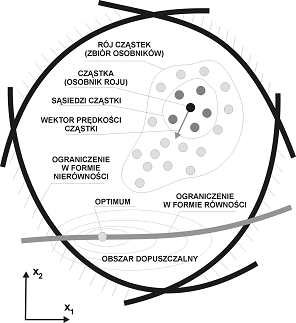
\includegraphics[width=.50\textwidth]{fig1.PNG}
    \caption{Podstawowe pojęcia PSO w 2D}
  \end{center}
\end{figure}
\end{document}
